\documentclass[aspectratio=169]{beamer}
\usefonttheme{serif}

\setbeamertemplate{navigation symbols}{}

\usepackage{amsmath}
\usepackage{enumitem}
\usepackage{bm}
\usepackage{ifthen}
\usepackage{listings}
\usepackage{xcolor}
\usepackage[most]{tcolorbox}
\usepackage{tikz}
\usetikzlibrary{arrows}
\usepackage{algorithm2e}
\usetikzlibrary{shapes.geometric}
\usetikzlibrary{overlay-beamer-styles}
\usepackage{booktabs}
\usepackage{mdframed}

\definecolor{codered}{HTML}{FB4933}
\definecolor{codegreen}{HTML}{A8C8A3}
\definecolor{codeorange}{HTML}{FE8019}
\definecolor{background}{HTML}{282828}

\lstset{
    language=C++,                
    backgroundcolor=\color{background},
    keywordstyle=\color{codered},
    basicstyle=\ttfamily\footnotesize,
    morekeywords=[2]{typedef, struct},
    morekeywords=[3]{int, Color, Node},
    morekeywords=[4]{RED, BLACK, data, color, left, right},
    keywordstyle=[2]\color{codered},
    keywordstyle=[3]\color{codeorange},
    keywordstyle=[4]\color{codegreen},
    literate=
    {*}{{\textcolor{codeorange}{*}}}1
    {,}{{\textcolor{codeorange}{,}}}1
    {\{}{{\textcolor{codeorange}{\{}}}1
    {\}}{{\textcolor{codeorange}{\}}}}1
    {;}{{\textcolor{codeorange}{;}}}1,
    numbersep=5pt,                  
    showspaces=false,                
    showstringspaces=false,
    showtabs=false,                  
    tabsize=2,
    frame=single
}

\tikzset{
    tnode/.style = {align=center, inner sep=0pt, text centered},
    node/.style = {tnode, circle, draw=black, text width=1.5em, thin},
    nnil/.style = {tnode, rectangle, draw=black, minimum width=1.5em, minimum height=1.5em, thin, scale=0.6},
    sub/.style = {isosceles triangle, draw=black, isosceles triangle apex angle=60, shape border uses incircle, anchor=north, shape border rotate=90, minimum height=1.5em, thin, scale=0.6}
}

\tikzset{
    treenode/.style = {align=center, inner sep=0pt, text centered},
    red_node/.style = {treenode, circle, white, draw=red, fill=red, text width=1.5em},
    black_node/.style = {treenode, circle, white, draw=black, fill=black, text width=1.5em, very thin},
    blue_node/.style = {treenode, circle, white, draw=blue, fill=blue, text width=1.5em, very thin},
    nil/.style = {treenode, rectangle, draw=black, fill=black, minimum width=1.5em, minimum height=1.5em, scale=0.6},
    bsub/.style = {isosceles triangle, white, draw=black, fill=black, isosceles triangle apex angle=60, shape border uses incircle, anchor=north, shape border rotate=90, minimum height=1.5em, thin, scale=0.6},
    rsub/.style = {isosceles triangle, white, draw=red, fill=red, isosceles triangle apex angle=60, shape border uses incircle, anchor=north, shape border rotate=90, minimum height=1.5em, thin, scale=0.6},
    esub/.style = {isosceles triangle, white, draw=blue, fill=blue, isosceles triangle apex angle=60, shape border uses incircle, anchor=north, shape border rotate=90, minimum height=1.5em, thin, scale=0.6}
}

\title{Balanced Trees (Red-Black Trees)}
\author{Warren Kim}
\date{}


\newcommand{\textib}[1]{\textit{\textbf{{#1}}}}
\newcommand{\red}{\textib{\color{red}{red }}}

\newcommand{\proposition}[1]{\begin{tcolorbox}[title={Proposition}]\small{\textit{{#1}}}\end{tcolorbox}}
\newcommand{\thm}[1]{\begin{tcolorbox}[title={Theorem}]\small{\textit{{#1}}}\end{tcolorbox}}
\newcommand{\define}[1]{\begin{tcolorbox}[title={Definition}]\small{\textit{{#1}}}\end{tcolorbox}}


\begin{document}

\maketitle

% ===== MOTIVATION =====
\begin{frame}{Motivation}
    \begin{enumerate}[label=\textit{(\roman*)}]
        \item Raw binary search tree performance is highly dependant on input order
        \item We want to ensure ${\cal{O}}(\log n)$ search, insertion, and deletion; i.e. predictable
            performance
    \end{enumerate}
\end{frame}

%===== EXAMPLE ===== 
\begin{frame}[fragile]{Example}
    Suppose we have the input set $\{1, 2, 3, 4, 5, 6, 7\}$ and consider two input orders:
    \newline
    \newline
    \begin{minipage}{.45\textwidth}
        \centering
        $\{1, 2, 3, 4, 5, 6, 7\}$ 
        \newline
        \newline
        \begin{tikzpicture}[-,>=stealth',level/.style={level distance = 0.8cm},
            edge from parent path={(\tikzparentnode) -- (\tikzchildnode.north)},
            grow'=down,every node/.style={node}, scale=0.8]

            \tikzstyle{ndl} = [nnil, scale=0.5]
            \tikzstyle{nd} = [scale=0.8]

            \newcommand{\nsa}{nd}
            \newcommand{\nsb}{nd}
            \newcommand{\nsc}{nd}
            \newcommand{\nsd}{nd}
            \newcommand{\nse}{nd}
            \newcommand{\nsf}{nd}
            \newcommand{\setns}[2]{
                \ifthenelse{\insertslidenumber=#1}{\renewcommand{#2}{ndl}}{}
            }
            \newcommand{\setnum}[1]{\ifthenelse{\insertslidenumber<#1}{}{#1}}
            \setns{1}{\nsa}
            \setns{2}{\nsb}
            \setns{3}{\nsc}
            \setns{4}{\nsd}
            \setns{5}{\nse}
            \setns{6}{\nsf}
            \node [scale=0.8]
            {1}
            child { 
                node [\nsa] {\setnum{2}}
                child [visible on=<2->] { 
                    node [\nsb] {\setnum{3}} 
                    child [visible on=<3->] { 
                        node [\nsc] {\setnum{4}} 
                        child [visible on=<4->] { 
                            node [\nsd] {\setnum{5}} 
                            child [visible on=<5->] { 
                                node [\nse] {\setnum{6}} 
                                child [visible on=<6->] { 
                                    node [\nsf] {\setnum{7}} 
                                    child [visible on=<7->] { node [nnil, scale=0.5] {} }
                                    child [visible on=<7->] { node [nnil, scale=0.5] {} }
                                }
                                child [visible on=<6->] { node [nnil, scale=0.5] {} }
                            }
                            child [visible on=<5->] { node [nnil, scale=0.5] {} }
                        }
                        child [visible on=<4->] { node [nnil, scale=0.5] {} }
                    }
                    child [visible on=<3->] { node [nnil, scale=0.5] {} }
                }
                child [visible on=<2->] { node [nnil, scale=0.5] {} }
            }
            child { 
                node [nnil, scale=0.5] {}
            }
            ;
        \end{tikzpicture}
    \end{minipage}
    \hfill
    \begin{minipage}{.45\textwidth}
        \centering
        $\{1, 7, 2, 6, 3, 5, 4\}$ 
        \newline
        \newline
        \begin{tikzpicture}[-,>=stealth',level/.style={sibling distance = 5cm/(#1 / 1.2), level distance = 0.8cm},
            edge from parent path={(\tikzparentnode) -- (\tikzchildnode.north)},
            grow'=down,every node/.style={node},scale=0.8]
            \tikzstyle{ndl} = [nnil, scale=0.5]
            \tikzstyle{nd} = [scale=0.8]

            \newcommand{\nsa}{nd}
            \newcommand{\nsb}{nd}
            \newcommand{\nsc}{nd}
            \newcommand{\nsd}{nd}
            \newcommand{\nse}{nd}
            \newcommand{\nsf}{nd}
            \newcommand{\setns}[2]{
                \pgfmathsetmacro{\result}{#1 + 7}
                \ifthenelse{\insertslidenumber<\result}{\renewcommand{#2}{ndl}}{}
            }
            \newcommand{\setnum}[2]{
                \ifthenelse{\equal{#2}{ndl}}{}{#1}
            }
            \setns{1}{\nsa}
            \setns{2}{\nsb}
            \setns{3}{\nsc}
            \setns{4}{\nsd}
            \setns{5}{\nse}
            \setns{6}{\nsf}

            \node [scale=0.8]
            {1}
            child { 
                node [\nsa] {\setnum{7}{\nsa}} 
                child [visible on=<8->] { node [nnil, scale=0.5] {} }
                child [visible on=<8->] { 
                    node [\nsb] {\setnum{2}{\nsb}} 
                    child [visible on=<9->] { 
                        node [\nsc] {\setnum{6}{\nsc}} 
                        child [visible on=<10->] { node [nnil, scale=0.5] {} }
                        child [visible on=<10->] { 
                            node [\nsd] {\setnum{3}{\nsd}} 
                            child [visible on=<11->] { 
                                node [\nse] {\setnum{5}{\nse}} 
                                child [visible on=<12->] { node [nnil, scale=0.5] {} }
                                child [visible on=<12->] { 
                                    node [\nsf] {\setnum{4}{\nsf}} 
                                    child [visible on=<13>] { node [nnil, scale=0.5] {} }
                                    child [visible on=<13>] { node [nnil, scale=0.5] {} }
                                }
                            }
                            child [visible on=<11->] { node [nnil, scale=0.5] {} }
                        }
                    }
                    child [visible on=<9->] { node [nnil, scale=0.5] {} }
                }
            }
            child { node [nnil, scale=0.5] {} }
            ;
        \end{tikzpicture}
    \end{minipage}
\end{frame}

% \begin{frame}[fragile]{Example: Input order \textit{(i)}}
%     \textit{(i)} $\{1, 2, 3, 4, 5, 6, 7\}$ 
%     \begin{center}
%         \begin{tikzpicture}[-,>=stealth',level/.style={level distance = 0.8cm},
%             edge from parent path={(\tikzparentnode) -- (\tikzchildnode.north)},grow'=down,every node/.style={node}]
%             \node 
%             {1}
%             child { 
%                 node {2}
%                 child { 
%                     node {3} 
%                     child { 
%                         node {4} 
%                         child { 
%                             node {5} 
%                             child { 
%                                 node {6} 
%                                 child { 
%                                     node {7} 
%                                     child { node [nnil] {} }
%                                     child { node [nnil] {} }
%                                 }
%                                 child { node [nnil] {} }
%                             }
%                             child { node [nnil] {} }
%                         }
%                         child { node [nnil] {} }
%                     }
%                     child { node [nnil] {} }
%                 }
%                 child { node [nnil] {} }
%             }
%             child { 
%                 node [nnil] {}
%             }
%             ;
%         \end{tikzpicture}
%     \end{center}
% \end{frame}

% \begin{frame}[fragile]{Example: Input order \textit{(ii)}}
%     \textit{(ii)} $\{1, 7, 2, 6, 3, 5, 4\}$ 
%     \begin{center}
%         \begin{tikzpicture}[-,>=stealth',level/.style={sibling distance = 5cm/(#1 / 1.5), level distance = 0.8cm},
%             edge from parent path={(\tikzparentnode) -- (\tikzchildnode.north)},grow'=down,every node/.style={node}]
%             \node 
%             {1}
%             child { 
%                 node {7} 
%                 child { node [nnil] {} }
%                 child { 
%                     node {2} 
%                     child { 
%                         node {6} 
%                         child { node [nnil] {} }
%                         child { 
%                             node {3} 
%                             child { 
%                                 node {5} 
%                                 child { node [nnil] {} }
%                                 child { 
%                                     node {4} 
%                                     child { node [nnil] {} }
%                                     child { node [nnil] {} }
%                                 }
%                             }
%                             child { node [nnil] {} }
%                         }
%                     }
%                     child { node [nnil] {} }
%                 }
%             }
%             child { node [nnil] {} }
%             ;
%         \end{tikzpicture}
%     \end{center}
% \end{frame}

% \begin{frame}[fragile]{Example: Input order \textit{(ii)}}
%     \textit{(ii)} $\{4, 2, 6, 1, 5, 3, 7\}$ 
%     \begin{center}
%         \begin{tikzpicture}[-,>=stealth',level/.style={sibling distance = 5cm/#1, level distance = 1.5cm},
%             edge from parent path={(\tikzparentnode) -- (\tikzchildnode.north)},grow'=down,every node/.style={node}]
%             \node 
%             {4}
%             child { 
%                 node {6} 
%                 child { 
%                     node {7} 
%                     child { node [nnil] {} }
%                     child { node [nnil] {} }
%                 }
%                 child { 
%                     node {5} 
%                     child { node [nnil] {} }
%                     child { node [nnil] {} }
%                 }
%             }
%             child { 
%                 node {2} 
%                 child { 
%                     node {3} 
%                     child { node [nnil] {} }
%                     child { node [nnil] {} }
%                 }
%                 child { 
%                     node {1} 
%                     child { node [nnil] {} }
%                     child { node [nnil] {} }
%                 }
%             }
%             ;
%         \end{tikzpicture}
%     \end{center}
% \end{frame}

% ===== INTUITION =====
\begin{frame}{Intuition}
    \textib{How do we balance binary trees?}
    \newline
    \newline
    \onslide<2-> {
        We can \textit{dynamically} balance the tree!
    }
    \newline
    \newline
    \onslide<3-> {
        We want to enforce a set of well-defined conditions. We can achieve this by adding
        additional member variables in our \texttt{Node} struct.
    }
\end{frame}

% ===== EXAMPLE =====
% \begin{frame}[fragile]{Example: Rotation around $2$}
%     \centering
%     \begin{minipage}{.4\textwidth}
%         \centering
%         \begin{tikzpicture}[-,>=stealth',level/.style={level distance = 0.8cm},
%             edge from parent path={(\tikzparentnode) -- (\tikzchildnode.north)},grow'=down,every node/.style={node}]
%             \node 
%             {1}
%             child { 
%                 node {2}
%                 child { 
%                     node {3} 
%                     child { node [nnil] {} }
%                     child { node [sub] {$\beta$} }
%                 }
%                 child { node [sub] {$\alpha$} }
%             }
%             child { 
%                 node [nnil] {}
%             }
%             ;
%         \end{tikzpicture}
%     \end{minipage}
%     \begin{minipage}{.1\textwidth}
%         \centering
%         \tikz \draw[-latex] (0,0) -- (1,0);
%     \end{minipage}
%     \begin{minipage}{.4\textwidth}
%         \centering
%         \begin{tikzpicture}[-,>=stealth',level/.style={sibling distance = 3cm/#1, level distance = 1cm},
%             edge from parent path={(\tikzparentnode) -- (\tikzchildnode.north)},grow'=down,every node/.style={node}]
%             \node 
%             {2}
%             child { 
%                 node {3}
%                 child { node [nnil] {} }
%                 child { node [sub] {$\beta$} }
%             }
%             child { 
%                 node {1} 
%                 child { node [sub] {$\alpha$} }
%                 child { node [nnil] {} }
%             }
%             ;
%         \end{tikzpicture}
%     \end{minipage}
% \end{frame}

% ===== DEFINITION =====
\begin{frame}[fragile]{Definition and Properties}
    \define{
        A \textib{\color{red}{red}}\textib{-black} tree is a type of \textib{self-balancing} binary 
        search tree that guarantees ${\cal{O}}(\log n)$ search, insertion, and deletion operations.
    }
    \begin{minipage}{.45\textwidth}
        \color{white}{
        \begin{enumerate}[label=\textit{(\roman*)}]
            \item \textit{Color:} Every node is either red or \textib{black}
            \item \textit{External:} All nil nodes are \textib{black}
            \item \textit{Internal:} A red node does not have a red child
            \item \textit{Depth:} Every path from the root to \textit{any} leaf node passes through
                the same number of \textib{black} nodes
            \item \textit{Root}: The root node is always \textib{black}
        \end{enumerate}
    }
    \end{minipage}
    \hfill
    \begin{minipage}{.5\textwidth}
        \begin{lstlisting}[backgroundcolor=\color{white}, frame=none]








        \end{lstlisting}    
    \end{minipage}
\end{frame}
% ===== DEFINITION =====
\begin{frame}[fragile]{Definition and Properties}
    \define{
        A \textib{\color{red}{red}}\textib{-black} tree is a type of \textib{self-balancing} binary 
        search tree that guarantees ${\cal{O}}(\log n)$ search, insertion, and deletion operations.
    }
    \begin{minipage}{.45\textwidth}
        \begin{enumerate}[label=\textit{(\roman*)}]
            \item \textit{Color:} Every node is either \red or \textib{black}
                \color{white}{
                \item \textit{External:} All nil nodes are \textib{black}
                \item \textit{Internal:} A red node does not have a red child
                \item \textit{Depth:} Every path from the root to \textit{any} leaf node passes through
                    the same number of \textib{black} nodes
                \item \textit{Root}: The root node is always \textib{black}
                }
        \end{enumerate}
    \end{minipage}
    \hfill
    \begin{minipage}{.5\textwidth}
        \begin{lstlisting}
typedef enum Color { RED, BLACK };

typedef struct Node {
    Color color;
    int data;
    Node *left;
    Node *right;
} Node;
        \end{lstlisting}    
    \end{minipage}
\end{frame}
% ===== DEFINITION =====
\begin{frame}[fragile]{Definition and Properties}
    \setbeamercovered{transparent=20}
    \define{
        A \textib{\color{red}{red}}\textib{-black} tree is a type of \textib{self-balancing} binary 
        search tree that guarantees ${\cal{O}}(\log n)$ search, insertion, and deletion operations.
    }
    \begin{minipage}{.45\textwidth}
        \begin{enumerate}[label=\textit{(\roman*)}]
            \item<0> \textit{Color:} Every node is either \red or \textib{black}
            \item \textit{External:} All nil nodes are \textib{black}
            \item[] \color{white}{\textit{Internal:} A red node does not have a red child}
                \color{white}{
                \item \textit{Depth:} Every path from the root to \textit{any} leaf node passes through
                    the same number of \textib{black} nodes
                \item \textit{Root}: The root node is always \textib{black}
                }
        \end{enumerate}
    \end{minipage}
    \hfill
    \begin{minipage}{.5\textwidth}
        \centering
        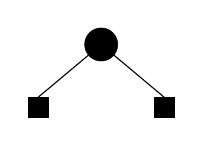
\begin{tikzpicture}[-,>=stealth',level/.style={sibling distance = 2cm/#1, level distance = 1cm},
            edge from parent path={(\tikzparentnode) -- (\tikzchildnode.north)}, scale=0.8]
            \node 
            [black_node, scale=0.8] {}
            child{ node [nil, scale=0.8] {}}
            child{ node [nil, scale=0.8] {}}
            ; 
        \end{tikzpicture}
        \newline
        \newline
        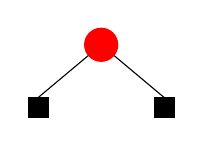
\begin{tikzpicture}[-,>=stealth',level/.style={sibling distance = 2cm/#1, level distance = 1cm},
            edge from parent path={(\tikzparentnode) -- (\tikzchildnode.north)}, scale=0.8]
            \node 
            [red_node, scale=0.8] {}
            child{ node [nil, scale=0.8] {}}
            child{ node [nil, scale=0.8] {}}
            ; 
        \end{tikzpicture}
    \end{minipage}
\end{frame}
% ===== DEFINITION =====
\begin{frame}[fragile]{Definition and Properties}
    \setbeamercovered{transparent=20}
    \define{
        A \textib{\color{red}{red}}\textib{-black} tree is a type of \textib{self-balancing} binary 
        search tree that guarantees ${\cal{O}}(\log n)$ search, insertion, and deletion operations.
    }
    \begin{minipage}{.45\textwidth}
        \begin{enumerate}[label=\textit{(\roman*)}]
            \item<0> \textit{Color:} Every node is either \red or \textib{black}
            \item<0> \textit{External:} All nil nodes are \textib{black}
            \item \textit{Internal:} A \red node does not have a \red child
                \color{white}{
                \item \textit{Depth:} Every path from the root to \textit{any} leaf node passes through
                    the same number of \textib{black} nodes
                \item \textit{Root}: The root node is always \textib{black}
                }
        \end{enumerate}
    \end{minipage}
    \hfill
    \begin{minipage}{.5\textwidth}
        \centering
        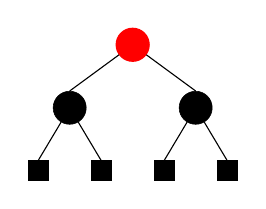
\begin{tikzpicture}[-,>=stealth',level/.style={sibling distance = 2cm/#1, level distance = 1cm},
            edge from parent path={(\tikzparentnode) -- (\tikzchildnode.north)}, scale=0.8]
            \node 
            [red_node, scale=0.8] {}
            child { 
                node [black_node, scale=0.8] {}
                child{ node [nil, scale=0.8] {}}
                child{ node [nil, scale=0.8] {}}
            }
            child { 
                node [black_node, scale=0.8] {}
                child{ node [nil, scale=0.8] {}}
                child{ node [nil, scale=0.8] {}}
            }
            ; 
        \end{tikzpicture}
        \textbf{Valid}
        \newline
        \newline
        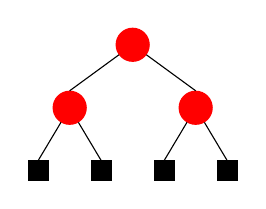
\begin{tikzpicture}[-,>=stealth',level/.style={sibling distance = 2cm/#1, level distance = 1cm},
            edge from parent path={(\tikzparentnode) -- (\tikzchildnode.north)}, scale=0.8]
            \node 
            [red_node, scale=0.8] {}
            child { 
                node [red_node, scale=0.8] {}
                child{ node [nil, scale=0.8] {}}
                child{ node [nil, scale=0.8] {}}
            }
            child { 
                node [red_node, scale=0.8] {}
                child{ node [nil, scale=0.8] {}}
                child{ node [nil, scale=0.8] {}}
            }
            ; 
        \end{tikzpicture}
        \textbf{\color{red}{Invalid}}
    \end{minipage}
\end{frame}
% ===== DEFINITION =====
\begin{frame}[fragile]{Definition and Properties}
    \setbeamercovered{transparent=20}
    \define{
        A \textib{\color{red}{red}}\textib{-black} tree is a type of \textib{self-balancing} binary 
        search tree that guarantees ${\cal{O}}(\log n)$ search, insertion, and deletion operations.
    }
    \begin{minipage}{.45\textwidth}
        \begin{enumerate}[label=\textit{(\roman*)}]
            \item<0> \textit{Color:} Every node is either \red or \textib{black}
            \item<0> \textit{External:} All nil nodes are \textib{black}
            \item<0> \textit{Internal:} A \red node does not have a \red child
            \item<0> \textit{Depth:} Every path from the root to \textit{any} leaf node passes through
                the same number of \textib{black} nodes
            \item \textit{Root}: The root node is always \textib{black}
        \end{enumerate}
    \end{minipage}
    \hfill
    \begin{minipage}{.5\textwidth}
        \centering
        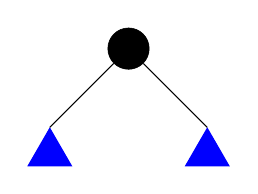
\begin{tikzpicture}[-,>=stealth',level/.style={sibling distance = 2cm/#1, level distance = 1cm},
            edge from parent path={(\tikzparentnode) -- (\tikzchildnode.north)}]
            \node 
            [black_node] {}
            child { 
                node [esub, scale=1.5] {}
            }
            child { 
                node [esub, scale=1.5] {}
            }
            ; 
        \end{tikzpicture}
    \end{minipage}
\end{frame}
% ===== DEFINITION =====
\begin{frame}[fragile]{Depth Property}
    \vspace{0.5cm}
    \textit{(iv) Depth:} Every path from the root to \textit{any} leaf node passes through the same number 
    of \textib{black} nodes
    \newline
    \begin{center}
        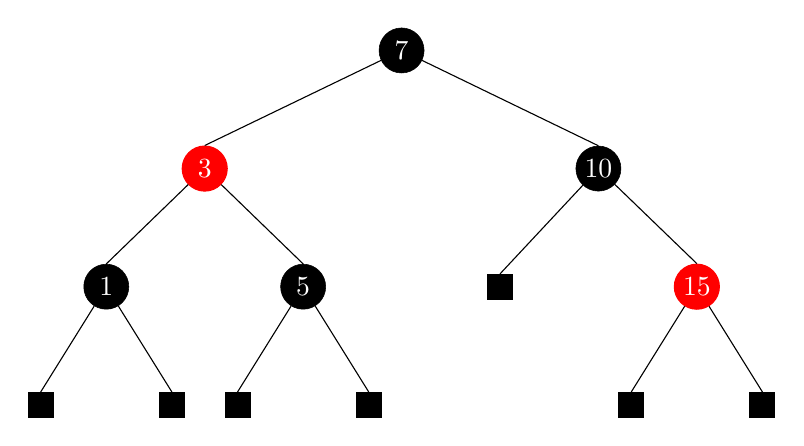
\begin{tikzpicture}[-,>=stealth',level/.style={sibling distance = 5cm/#1, level distance = 1.5cm},
            edge from parent path={(\tikzparentnode) -- (\tikzchildnode.north)}]
            \node [black_node] {7}
            child{ node [red_node] {3} 
                child{ node [black_node] {1} 
                    child{ node [nil] {} }
                    child{ node [nil] {} }
                }
                child{ node [black_node] {5}
                    child{ node [nil] {} }
                    child{ node [nil] {} }
                }                            
            }
            child{ node [black_node] {10}
                child{ node [nil] {} }
                child{ node [red_node] {15}
                    child{ node [nil] {} }
                    child{ node [nil] {} }
                }
            }
            ; 
        \end{tikzpicture}
    \end{center}
\end{frame}
% ===== DEFINITION =====
\begin{frame}[fragile]{Depth Property}
    \textit{(iv) Depth:} Every path from the root to \textit{any} leaf node passes through the same number 
    of \textib{black} nodes
    \newline
    \begin{center}
        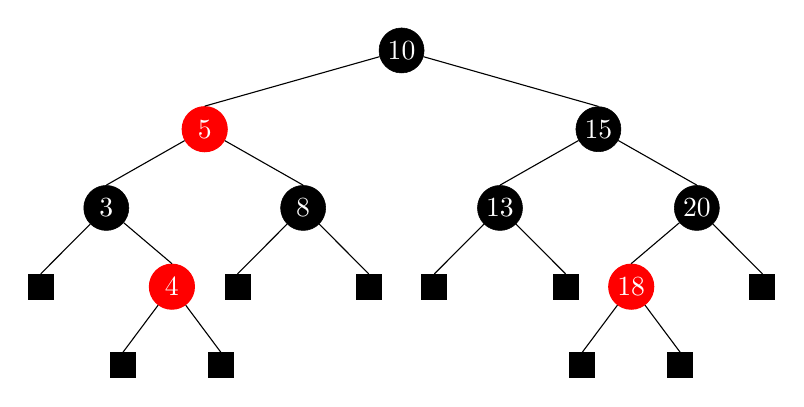
\begin{tikzpicture}[-,>=stealth',level/.style={sibling distance = 5cm/#1, level distance = 1cm},
            edge from parent path={(\tikzparentnode) -- (\tikzchildnode.north)}]
            \node [black_node] {10}
            child{ node [red_node] {5} 
                child{ node [black_node] {3} 
                    child{ node [nil] {} }
                    child{ node [red_node] {4}
                        child{ node [nil] {} }
                        child{ node [nil] {} }
                    }
                }
                child{ node [black_node] {8}
                    child{ node [nil] {} }
                    child{ node [nil] {} }
                }                            
            }
            child{ node [black_node] {15}
                child{ node [black_node] {13} 
                    child{ node [nil] {} }
                    child{ node [nil] {} }
                }
                child{ node [black_node] {20}
                    child{ node [red_node] {18}
                        child{ node [nil] {} }
                        child{ node [nil] {} }
                    }
                    child{ node [nil] {} }
                }
            }
            ;
        \end{tikzpicture}
    \end{center}
\end{frame}
% ===== DEFINITION =====
\begin{frame}[fragile]{Depth Property}
    \textit{(iv) Depth:} Every path from the root to \textit{any} leaf node passes through the same number 
    of \textib{black} nodes
    \newline
    \begin{center}
        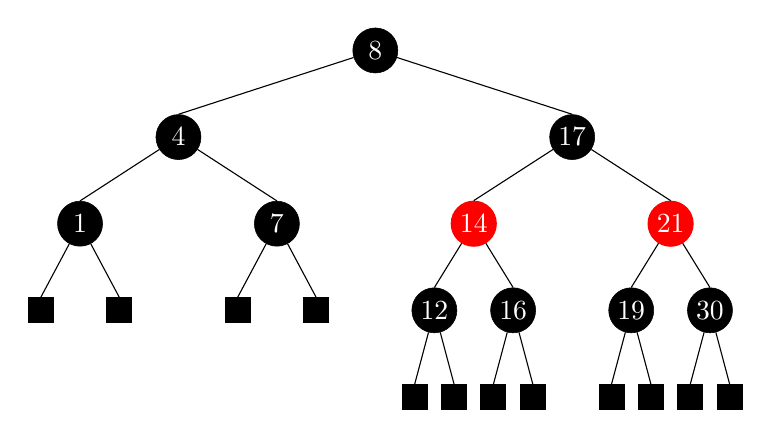
\begin{tikzpicture}[-,>=stealth',level/.style={sibling distance = 10cm/(#1 / 0.5), level distance = 1.1cm},
            edge from parent path={(\tikzparentnode) -- (\tikzchildnode.north)},
            level 3/.style={sibling distance=10mm},
            level 4/.style={sibling distance=5mm}]
            \node [black_node] {8}
            child{ node [black_node] {4} 
                child{ node [black_node] {1} 
                    child{ node [nil] {} }
                    child{ node [nil] {} }
                }
                child{ node [black_node] {7}
                    child{ node [nil] {} }
                    child{ node [nil] {} }
                }                            
            }
            child{ node [black_node] {17}
                child{ node [red_node] {14} 
                    child{ node [black_node] {12}
                        child{ node [nil] {14} }
                        child{ node [nil] {} }
                    }                            
                    child{ node [black_node] {16}
                        child{ node [nil] {} }
                        child{ node [nil] {} }
                    }                            
                }
                child{ node [red_node] {21}
                    child{ node [black_node] {19}
                        child{ node [nil] {} }
                        child{ node [nil] {} }
                    }
                    child{ node [black_node] {30}
                        child{ node [nil] {} }
                        child{ node [nil] {} }
                    }                            
                }
            }
            ;
        \end{tikzpicture}
    \end{center}
\end{frame}
% ===== DEFINITION =====
\begin{frame}[fragile]{Definition and Properties}
    \define{
        A \textib{\color{red}{red}}\textib{-black} tree is a type of \textib{self-balancing} binary 
        search tree that guarantees ${\cal{O}}(\log n)$ search, insertion, and deletion operations.
    }
    \begin{enumerate}[label=\textit{(\roman*)}]
        \item \textit{Color:} Every node is either \red or \textib{black}
        \item \textit{External:} All nil nodes are \textib{black}
        \item \textit{Internal:} A \red node does not have a \red child
        \item \textit{Depth:} Every path from the root to \textit{any} leaf node passes through
            the same number of \textib{black} nodes
        \item \textit{Root}: The root node is always \textib{black}
    \end{enumerate}
\end{frame}

\begin{frame}{Insertion}
    Suppose we have a node $z$ to insert into our red-black tree. Then,
    \begin{enumerate}[label=\textit{(\roman*)}]
        \item Like a BST, insert $z$.
        \item Color $z$ \red.
        \item Fix double \red violations, if any.
        \item Recursively (or iteratively) fix violations.
    \end{enumerate}
\end{frame}

\begin{frame}{Double Red Violations}
    Recall \textit{Property (iii): A \red node does not have a \red child}. 
    \newline
    There are two cases:
    \begin{enumerate}[label=\textit{(\roman*)}]
        \item \textib{Recolor:} If both the \textit{parent} and \textit{uncle} are 
            \textib{\color{red}{red}}, perform a \textit{recolor}.
        \item \textib{Restructure:} If the \textit{parent} is \red but the \textit{uncle} is 
            \textib{black}, perform a \textit{tri-node restructure}.
    \end{enumerate}
\end{frame}

\begin{frame}[fragile]{Recolor}
    \begin{center}
        \begin{minipage}{.4\textwidth}
            \begin{center}
                \begin{tikzpicture}[-,>=stealth',level/.style={sibling distance = 3cm/#1, level distance = 1cm},
                    edge from parent path={(\tikzparentnode) -- (\tikzchildnode.north)}]
                    \tikzstyle{ndl} = [nil]
                    \tikzstyle{nd} = [red_node]

                    \newcommand{\ns}{nd}
                    \newcommand{\setns}[1]{
                        \ifthenelse{\insertslidenumber=1}{\renewcommand{\ns}{ndl}}{}
                    }
                    \newcommand{\setnum}[1]{
                        \ifthenelse{\insertslidenumber=1}{}{#1}
                    }
                    \setns{1}

                    \node 
                    [black_node] {$u$}
                    child{ 
                        node [red_node] {$w$} 
                        child { node [bsub] {} }
                        child { node [bsub] {} }
                    }
                    child{ 
                        node [red_node] {$v$}
                        child { 
                            node [\ns] {\setnum{$z$}}
                            child [visible on=<2->] { node [nil] {}}
                            child [visible on=<2->] { node [nil] {}}
                        }
                        child { node [bsub] {} }
                    }
                    ; 
                \end{tikzpicture}
            \end{center}
        \end{minipage}
        \onslide<3>{
            \begin{minipage}{.1\textwidth}
                \begin{center}
                    \tikz \draw[-latex] (0,0) -- (1,0);
                \end{center}
            \end{minipage}
            \begin{minipage}{.4\textwidth}
                \begin{center}
                    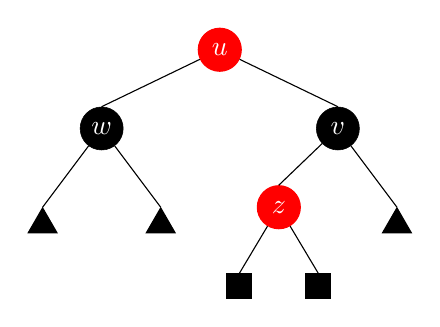
\begin{tikzpicture}[-,>=stealth',level/.style={sibling distance = 3cm/#1, level distance = 1cm},
                        edge from parent path={(\tikzparentnode) -- (\tikzchildnode.north)}]
                    \node 
                    [red_node] {$u$}
                    child{ 
                        node [black_node] {$w$} 
                        child { node [bsub] {} }
                        child { node [bsub] {} }
                    }
                    child{ 
                        node [black_node] {$v$}
                        child{ 
                            node [red_node] {$z$}
                            child{ node [nil] {}}
                            child{ node [nil] {}}
                        }
                        child { node [bsub] {} }
                    }
                    ; 
                    \end{tikzpicture}
                \end{center}
            \end{minipage}
        }
    \end{center}
    where
    \begin{enumerate}[label=, leftmargin=*]
        \item $z$ is the new node
        \item $v$ is $z$'s parent
        \item $u$ is $z$'s grandparent
        \item $w$ is $z$'s uncle
    \end{enumerate}

\end{frame}

\begin{frame}{Tri-Node Restructure}
    There are four cases:
    \begin{enumerate}[label=\textit{(\roman*)}]
        \item Left-Left
        \item Right-Right
        \item Left-Right
        \item Right-Left
    \end{enumerate}
\end{frame}

\begin{frame}[fragile]{Case: Left-Left}
    \begin{center}
        \begin{minipage}{.4\textwidth}
            \begin{center}
                \begin{tikzpicture}[-,>=stealth',level/.style={sibling distance = 2.8cm/#1, level distance = 1cm},
                    edge from parent path={(\tikzparentnode) -- (\tikzchildnode.north)}]
                    \tikzstyle{ndl} = [nil]
                    \tikzstyle{nd} = [red_node]

                    \newcommand{\ns}{nd}
                    \newcommand{\setns}[1]{
                        \ifthenelse{\insertslidenumber=1}{\renewcommand{\ns}{ndl}}{}
                    }
                    \newcommand{\setnum}[1]{
                        \ifthenelse{\insertslidenumber=1}{}{#1}
                    }
                    \setns{1}

                    \node 
                    [black_node] {$u$}
                    child{ 
                        node [red_node] {$v$}
                        child{ 
                            node [\ns] {\setnum{$z$}}
                            child [visible on=<2->] { node [nil] {}}
                            child [visible on=<2->] { node [nil] {}}
                        }
                        child { node [bsub] {$T$} }
                    }
                    child{ 
                        node [black_node] {$w$} 
                        child { node [esub] {} }
                        child { node [esub] {} }
                    }
                    ; 
                \end{tikzpicture}
            \end{center}
        \end{minipage}
        \onslide<3>{
            \begin{minipage}{.1\textwidth}
                \begin{center}
                    \tikz \draw[-latex] (0,0) -- (1,0);
                \end{center}
            \end{minipage}
            \begin{minipage}{.4\textwidth}
                \begin{center}
                    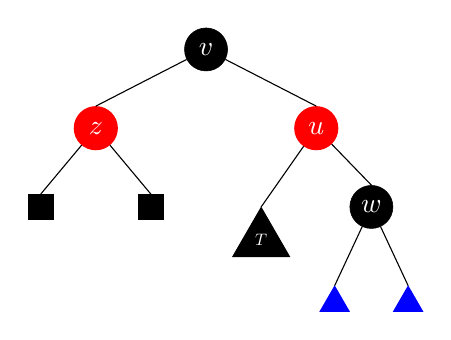
\begin{tikzpicture}[-,>=stealth',level/.style={sibling distance = 2.8cm/#1, level distance = 1cm},
                        edge from parent path={(\tikzparentnode) -- (\tikzchildnode.north)}]
                        \node 
                        [black_node] {$v$}
                        child{ 
                            node [red_node] {$z$}
                            child{ node [nil] {}}
                            child{ node [nil] {}}
                        }
                        child{ 
                            node [red_node] {$u$} 
                            child { node [bsub] {$T$} }
                            child{ 
                                node [black_node] {$w$}
                                child { node [esub] {} }
                                child { node [esub] {} }
                            }
                        }
                        ; 
                    \end{tikzpicture}
                \end{center}
            \end{minipage}
        }
    \end{center}
    where
    \begin{enumerate}[label=,leftmargin=*]
        \item $z$ is the new node
        \item $v$ is $z$'s parent
        \item $u$ is $z$'s grandparent
        \item $w$ is $z$'s uncle
        \item $T$ is $v$'s subtree
    \end{enumerate}
\end{frame}

\begin{frame}[fragile]{Case: Right-Right}
    \begin{center}
        \begin{minipage}{.4\textwidth}
            \begin{center}
                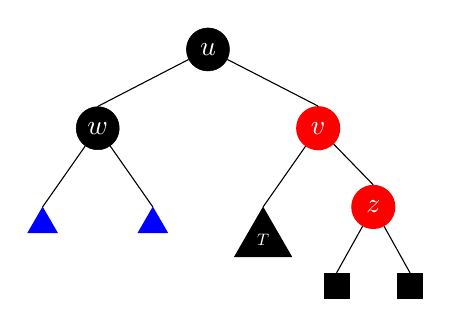
\begin{tikzpicture}[-,>=stealth',level/.style={sibling distance = 2.8cm/#1, level distance = 1cm},
                    edge from parent path={(\tikzparentnode) -- (\tikzchildnode.north)}]
                    \node 
                    [black_node] {$u$}
                    child{ 
                        node [black_node] {$w$} 
                        child { node [esub] {} }
                        child { node [esub] {} }
                    }
                    child{ 
                        node [red_node] {$v$}
                        child { node [bsub] {$T$} }
                        child{ 
                            node [red_node] {$z$}
                            child{ node [nil] {}}
                            child{ node [nil] {}}
                        }
                    }
                    ; 
                \end{tikzpicture}
            \end{center}
        \end{minipage}
        \begin{minipage}{.1\textwidth}
            \begin{center}
                \tikz \draw[-latex] (0,0) -- (1,0);
            \end{center}
        \end{minipage}
        \begin{minipage}{.4\textwidth}
            \begin{center}
                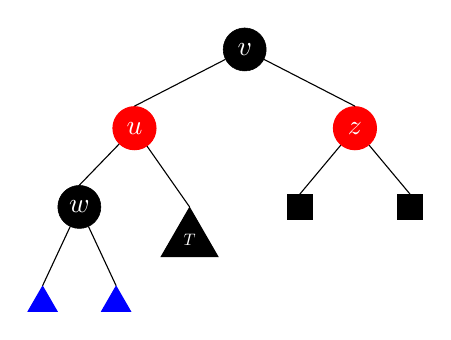
\begin{tikzpicture}[-,>=stealth',level/.style={sibling distance = 2.8cm/#1, level distance = 1cm},
                    edge from parent path={(\tikzparentnode) -- (\tikzchildnode.north)}]
                    \node 
                    [black_node] {$v$}
                    child{ 
                        node [red_node] {$u$}
                        child{ 
                            node [black_node] {$w$}
                            child { node [esub] {} }
                            child { node [esub] {} }
                        }
                        child { node [bsub] {$T$} }
                    }
                    child{ 
                        node [red_node] {$z$} 
                        child{ node [nil] {}}
                        child{ node [nil] {}}
                    }
                    ; 
                \end{tikzpicture}
            \end{center}
        \end{minipage}
    \end{center}
    where
    \begin{enumerate}[label=,leftmargin=*]
        \item $z$ is the new node
        \item $v$ is $z$'s parent
        \item $u$ is $z$'s grandparent
        \item $w$ is $z$'s uncle
        \item $T$ is $v$'s subtree
    \end{enumerate}
\end{frame}

\begin{frame}[fragile]{Case: Left-Right}
    \begin{center}
        \begin{minipage}{.4\textwidth}
            \begin{center}
                \begin{tikzpicture}[-,>=stealth',level/.style={sibling distance = 2.8cm/#1, level distance = 1cm},
                    edge from parent path={(\tikzparentnode) -- (\tikzchildnode.north)}]
                    \tikzstyle{ndl} = [nil]
                    \tikzstyle{nd} = [red_node]

                    \newcommand{\ns}{nd}
                    \newcommand{\setns}[1]{
                        \ifthenelse{\insertslidenumber=1}{\renewcommand{\ns}{ndl}}{}
                    }
                    \newcommand{\setnum}[1]{
                        \ifthenelse{\insertslidenumber=1}{}{#1}
                    }
                    \setns{1}

                    \node 
                    [black_node] {$u$}
                    child{ 
                        node [red_node] {$v$}
                        child { node [bsub] {$T$} }
                        child{ 
                            node [\ns] {\setnum{$z$}}
                            child [visible on=<2->] { node [nil] {}}
                            child [visible on=<2->] { node [nil] {}}
                        }
                    }
                    child{ 
                        node [black_node] {$w$} 
                        child { node [esub] {} }
                        child { node [esub] {} }
                    }
                    ; 
                \end{tikzpicture}
            \end{center}
        \end{minipage}
        \onslide<3>{
            \begin{minipage}{.1\textwidth}
                \begin{center}
                    \tikz \draw[-latex] (0,0) -- (1,0);
                \end{center}
            \end{minipage}
            \begin{minipage}{.4\textwidth}
                \begin{center}
                    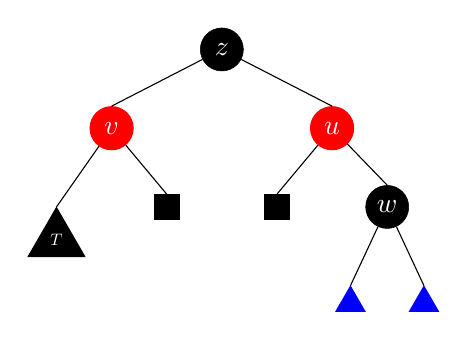
\begin{tikzpicture}[-,>=stealth',level/.style={sibling distance = 2.8cm/#1, level distance = 1cm},
                        edge from parent path={(\tikzparentnode) -- (\tikzchildnode.north)}]
                        \node 
                        [black_node] {$z$}
                        child{ 
                            node [red_node] {$v$}
                            child { node [bsub] {$T$} }
                            child{ node [nil] {}}
                        }
                        child{ 
                            node [red_node] {$u$} 
                            child{ node [nil] {}}
                            child{ 
                                node [black_node] {$w$}
                                child { node [esub] {} }
                                child { node [esub] {} }
                            }
                        }
                        ; 
                    \end{tikzpicture}
                \end{center}
            \end{minipage}
        }
    \end{center}
    where
    \begin{enumerate}[label=,leftmargin=*]
        \item $z$ is the new node
        \item $v$ is $z$'s parent
        \item $u$ is $z$'s grandparent
        \item $w$ is $z$'s uncle
        \item $T$ is $v$'s subtree
    \end{enumerate}
\end{frame}

\begin{frame}[fragile]{Case: Right-Left}
    \begin{center}
        \begin{minipage}{.4\textwidth}
            \begin{center}
                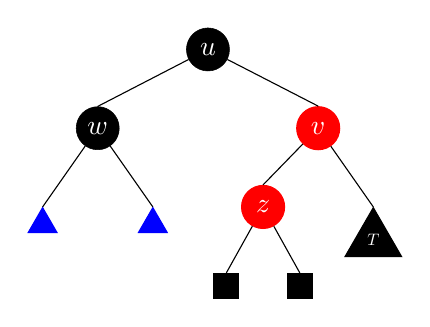
\begin{tikzpicture}[-,>=stealth',level/.style={sibling distance = 2.8cm/#1, level distance = 1cm},
                    edge from parent path={(\tikzparentnode) -- (\tikzchildnode.north)}]
                    \node 
                    [black_node] {$u$}
                    child{ 
                        node [black_node] {$w$} 
                        child { node [esub] {} }
                        child { node [esub] {} }
                    }
                    child{ 
                        node [red_node] {$v$}
                        child{ 
                            node [red_node] {$z$}
                            child{ node [nil] {}}
                            child{ node [nil] {}}
                        }
                        child { node [bsub] {$T$} }
                    }
                    ; 
                \end{tikzpicture}
            \end{center}
        \end{minipage}
        \begin{minipage}{.1\textwidth}
            \begin{center}
                \tikz \draw[-latex] (0,0) -- (1,0);
            \end{center}
        \end{minipage}
        \begin{minipage}{.4\textwidth}
            \begin{center}
                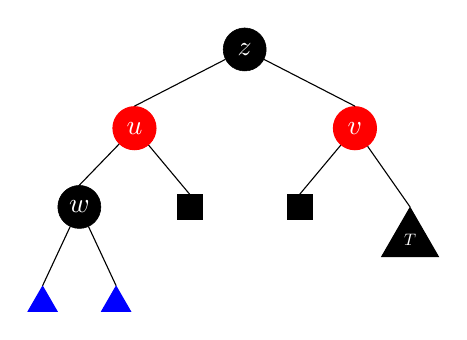
\begin{tikzpicture}[-,>=stealth',level/.style={sibling distance = 2.8cm/#1, level distance = 1cm},
                    edge from parent path={(\tikzparentnode) -- (\tikzchildnode.north)}]
                    \node 
                    [black_node] {$z$}
                    child{ 
                        node [red_node] {$u$} 
                        child{ 
                            node [black_node] {$w$}
                            child { node [esub] {} }
                            child { node [esub] {} }
                        }
                        child{ node [nil] {}}
                    }
                    child{ 
                        node [red_node] {$v$}
                        child{ node [nil] {}}
                        child { node [bsub] {$T$} }
                    }
                    ; 
                \end{tikzpicture}
            \end{center}
        \end{minipage}
    \end{center}
    where
    \begin{enumerate}[label=,leftmargin=*]
        \item $z$ is the new node
        \item $v$ is $z$'s parent
        \item $u$ is $z$'s grandparent
        \item $w$ is $z$'s uncle
        \item $T$ is $v$'s subtree
    \end{enumerate}
\end{frame}

% \begin{frame}{Deletion}
%     Suppose we have a node $z$ to delete from our red-black tree.
%     \newline
%     \begin{enumerate}[label=\textit{(\roman*)}]
%         \item If $z$ is a \red leaf node, simply remove $z$.
%         \item If $z$ only has a left child $s$, swap \textit{values} and remove $s$.
%         \item If $z$ has a right child, swap its \textit{value} with its in-order successor $s$ and 
%             remove $s$. 
%     \end{enumerate}
%     \hfil
%     \newline
%     If there is a double \textib{black} in \textit{(ii)} or \textit{(iii)}, perform a 
%     \textit{fixup} at $y$'s original position.
% \end{frame}

% \begin{frame}{Deletion Fixup}
%     There are three cases:
%     \begin{enumerate}[label=\textit{(\roman*)}]
%         \item $y$ has a \red child. Then, we perform a \textib{restructure}.
%         \item $y$'s sibling $w$ is \textib{black}. Then, we perform a \textib{recolor}.
%         \item $y$'s sibling $w$ is \red. Then, we perform an \textib{adjustment} followed by 
%             either case \textit{(ii)} or \textit{(iii)}.
%     \end{enumerate}
% \end{frame}

% \begin{frame}[fragile]{Restructure}
%     \begin{center}
%         \begin{minipage}{.4\textwidth}
%             \begin{center}
%                 \begin{tikzpicture}[-,>=stealth',level/.style={sibling distance = 2.8cm/#1, level distance = 1cm},
%                     edge from parent path={(\tikzparentnode) -- (\tikzchildnode.north)}]
%                     \node 
%                     [black_node] {$x$}
%                     child { 
%                         node [black_node] {$z$} 
%                         child { node [nil] {} }
%                         child { node [nil] {} }
%                     }
%                     child { 
%                         node [black_node] {$y$} 
%                         child { node [nil] {} }
%                         child { 
%                             node [red_node] {$c$} 
%                             child { node [nil] {} }
%                             child { node [nil] {} }
%                         }
%                     }
%                     ; 
%                 \end{tikzpicture}
%             \end{center}
%         \end{minipage}
%         \onslide<2>{
%             \begin{minipage}{.1\textwidth}
%                 \begin{center}
%                     \tikz \draw[-latex] (0,0) -- (1,0);
%                 \end{center}
%             \end{minipage}
%             \begin{minipage}{.4\textwidth}
%                 \begin{center}
%                     \begin{tikzpicture}[-,>=stealth',level/.style={sibling distance = 2.8cm/#1, level distance = 1cm},
%                         edge from parent path={(\tikzparentnode) -- (\tikzchildnode.north)}]
%                         \node 
%                         [black_node] {$y$}
%                         child { 
%                             node [black_node] {$x$} 
%                             child { node [nil] {} }
%                             child { node [nil] {} }
%                         }
%                         child { 
%                             node [black_node] {$c$} 
%                             child { node [nil] {} }
%                             child { node [nil] {} }
%                         }
%                         ; 
%                     \end{tikzpicture}
%                 \end{center}
%             \end{minipage}
%         }
%     \end{center}
%     where
%     \begin{enumerate}[label=,leftmargin=*]
%         \item $z$ is the node to delete
%         \item $y$ is $z$'s sibling 
%         \item $x$ is $y$'s parent
%         \item $c$ is $y$'s child
%     \end{enumerate}
% \end{frame}

% \begin{frame}[fragile]{Restructure}
%     \begin{center}
%         \begin{minipage}{.4\textwidth}
%             \begin{center}
%                 \begin{tikzpicture}[-,>=stealth',level/.style={sibling distance = 2.8cm/#1, level distance = 1cm},
%                     edge from parent path={(\tikzparentnode) -- (\tikzchildnode.north)}]
%                     \node 
%                     [black_node] {$x$}
%                     child { 
%                         node [black_node] {$z$} 
%                         child { node [nil] {} }
%                         child { node [nil] {} }
%                     }
%                     child { 
%                         node [black_node] {$y$} 
%                         child { 
%                             node [red_node] {$c$} 
%                             child { node [nil] {} }
%                             child { node [nil] {} }
%                         }
%                         child { node [nil] {} }
%                     }
%                     ; 
%                 \end{tikzpicture}
%             \end{center}
%         \end{minipage}
%         \onslide<2>{
%             \begin{minipage}{.1\textwidth}
%                 \begin{center}
%                     \tikz \draw[-latex] (0,0) -- (1,0);
%                 \end{center}
%             \end{minipage}
%             \begin{minipage}{.4\textwidth}
%                 \begin{center}
%                     \begin{tikzpicture}[-,>=stealth',level/.style={sibling distance = 2.8cm/#1, level distance = 1cm},
%                         edge from parent path={(\tikzparentnode) -- (\tikzchildnode.north)}]
%                         \node 
%                         [black_node] {$c$}
%                         child { 
%                             node [black_node] {$x$} 
%                             child { node [nil] {} }
%                             child { node [nil] {} }
%                         }
%                         child { 
%                             node [black_node] {$y$} 
%                             child { node [nil] {} }
%                             child { node [nil] {} }
%                         }
%                         ; 
%                     \end{tikzpicture}
%                 \end{center}
%             \end{minipage}
%         }
%     \end{center}
%     where
%     \begin{enumerate}[label=,leftmargin=*]
%         \item $z$ is the node to delete
%         \item $y$ is $z$'s sibling 
%         \item $x$ is $y$'s parent
%         \item $c$ is $y$'s child
%     \end{enumerate}
% \end{frame}



% \begin{frame}[fragile]{Recolor}
%     \begin{center}
%         \begin{minipage}{.4\textwidth}
%             \begin{center}
%                 \begin{tikzpicture}[-,>=stealth',level/.style={sibling distance = 2.8cm/#1, level distance = 1cm},
%                     edge from parent path={(\tikzparentnode) -- (\tikzchildnode.north)}]
%                     \node 
%                     [red_node] {$x$}
%                     child { 
%                         node [black_node] {$y$} 
%                         child { node [nil] {} }
%                         child { node [nil] {} }
%                     }
%                     child { 
%                         node [black_node] {$z$} 
%                         child { node [nil] {} }
%                         child { node [nil] {} }
%                     }
%                     ; 
%                 \end{tikzpicture}
%             \end{center}
%         \end{minipage}
%         \onslide<2>{
%             \begin{minipage}{.1\textwidth}
%                 \begin{center}
%                     \tikz \draw[-latex] (0,0) -- (1,0);
%                 \end{center}
%             \end{minipage}
%             \begin{minipage}{.4\textwidth}
%                 \begin{center}
%                     \begin{tikzpicture}[-,>=stealth',level/.style={sibling distance = 2.8cm/#1, level distance = 1cm},
%                         edge from parent path={(\tikzparentnode) -- (\tikzchildnode.north)}]
%                         \node 
%                         [black_node] {$x$}
%                         child { 
%                             node [red_node] {$y$} 
%                             child { node [nil] {} }
%                             child { node [nil] {} }
%                         }
%                         child { node [nil] {} }
%                         ; 
%                     \end{tikzpicture}
%                 \end{center}
%             \end{minipage}
%         }
%     \end{center}
%     where
%     \begin{enumerate}[label=,leftmargin=*]
%         \item $z$ is the node to delete
%         \item $y$ is $z$'s sibling 
%         \item $x$ is $y$'s parent
%         \item $c$ is $y$'s child
%     \end{enumerate}
% \end{frame}

% \begin{frame}[fragile]{Adjustment}
%     \begin{center}
%         \begin{minipage}{.4\textwidth}
%             \begin{center}
%                 \begin{tikzpicture}[-,>=stealth',level/.style={sibling distance = 2.8cm/#1, level distance = 1cm},
%                     edge from parent path={(\tikzparentnode) -- (\tikzchildnode.north)}]
%                     \node 
%                     [black_node] {$x$}
%                     child { 
%                         node [red_node] {$y$} 
%                         child { 
%                             node [black_node] {$c$} 
%                             child { node [nil] {} }
%                             child { node [nil] {} }
%                         }
%                         child { node [bsub] {$T$} }
%                     }
%                     child { 
%                         node [black_node] {$z$} 
%                         child { node [nil] {} }
%                         child { node [nil] {} }
%                     }
%                     ; 
%                 \end{tikzpicture}
%             \end{center}
%         \end{minipage}
%         \onslide<2>{
%             \begin{minipage}{.1\textwidth}
%                 \begin{center}
%                     \tikz \draw[-latex] (0,0) -- (1,0);
%                 \end{center}
%             \end{minipage}
%             \begin{minipage}{.4\textwidth}
%                 \begin{center}
%                     \begin{tikzpicture}[-,>=stealth',level/.style={sibling distance = 2.8cm/#1, level distance = 1cm},
%                         edge from parent path={(\tikzparentnode) -- (\tikzchildnode.north)}]
%                         \node 
%                         [black_node] {$y$}
%                         child { 
%                             node [black_node] {$c$} 
%                             child { node [nil] {} }
%                             child { node [nil] {} }
%                         }
%                         child { 
%                             node [black_node] {$x$} 
%                             child { node [rsub] {$T$} }
%                             child { node [nil] {} }
%                         }
%                         ; 
%                     \end{tikzpicture}
%                 \end{center}
%             \end{minipage}
%         }
%     \end{center}
%     where
%     \begin{enumerate}[label=,leftmargin=*]
%         \item $z$ is the node to delete
%         \item $y$ is $z$'s sibling 
%         \item $x$ is $y$'s parent
%         \item $c$ is $y$'s child
%     \end{enumerate}
% \end{frame}

% \begin{frame}[fragile]{Case: $y$ is a Leaf Node or has Two \textib{Black} Children}
%     \begin{center}
%         \begin{minipage}{.4\textwidth}
%             \begin{center}
%                 \begin{tikzpicture}[-,>=stealth',level/.style={sibling distance = 2.8cm/#1, level distance = 1cm},
%                     edge from parent path={(\tikzparentnode) -- (\tikzchildnode.north)}]
%                     \node 
%                     [black_node] {$x$}
%                     child{ 
%                         node [black_node] {$y$} 
%                         child { node [nil] {} }
%                         child { node [nil] {} }
%                     }
%                     child{ 
%                         node [black_node] {$w$}
%                         child { node [nil] {} }
%                         child { node [nil] {} }
%                     }
%                     ; 
%                 \end{tikzpicture}
%             \end{center}
%         \end{minipage}
%         \onslide<2>{
%             \begin{minipage}{.1\textwidth}
%                 \begin{center}
%                     \tikz \draw[-latex] (0,0) -- (1,0);
%                 \end{center}
%             \end{minipage}
%             \begin{minipage}{.4\textwidth}
%                 \begin{center}
%                     \begin{tikzpicture}[-,>=stealth',level/.style={sibling distance = 2.8cm/#1, level distance = 1cm},
%                         edge from parent path={(\tikzparentnode) -- (\tikzchildnode.north)}]
%                         \node 
%                         [black_node] {$x$}
%                         child { node [nil] {} }
%                         child{ 
%                             node [red_node] {$w$}
%                             child { node [nil] {} }
%                             child { node [nil] {} }
%                         }
%                         ; 
%                     \end{tikzpicture}
%                 \end{center}
%             \end{minipage}
%         }
%     \end{center}
%     where
%     \begin{enumerate}[label=,leftmargin=*]
%         \item $y$ is the node to delete
%         \item $w$ is $y$'s sibling
%         \item $x$ is $y$'s parent
%     \end{enumerate}
% \end{frame}

% \begin{frame}[fragile]{Case: $y$ has a \textib{\color{red}{Red}} Child}
%     \begin{center}
%         \begin{minipage}{.4\textwidth}
%             \begin{center}
%                 \begin{tikzpicture}[-,>=stealth',level/.style={sibling distance = 2.8cm/#1, level distance = 1cm},
%                     edge from parent path={(\tikzparentnode) -- (\tikzchildnode.north)}, scale=0.7]
%                     \node 
%                     [blue_node, scale=0.7] {$x$}
%                     child{ 
%                         node [black_node, scale=0.7] {$y$} 
%                         child { 
%                             node [red_node, scale=0.7] {$z$} 
%                             child { node [nil, scale=0.7] {} }
%                             child { node [nil, scale=0.7] {} }
%                         }
%                         child { node [nil, scale=0.7] {} }
%                     }
%                     child{ 
%                         node [black_node, scale=0.7] {$w$}
%                         child { node [nil, scale=0.7] {} }
%                         child { node [nil, scale=0.7] {} }
%                     }
%                     ; 
%                 \end{tikzpicture}
%                 \begin{tikzpicture}[-,>=stealth',level/.style={sibling distance = 2.8cm/#1, level distance = 1cm},
%                     edge from parent path={(\tikzparentnode) -- (\tikzchildnode.north)}, scale=0.7]
%                     \node 
%                     [blue_node, scale=0.7] {$x$}
%                     child{ 
%                         node [black_node, scale=0.7] {$y$} 
%                         child { node [nil, scale=0.7] {} }
%                         child { 
%                             node [red_node, scale=0.7] {$z$} 
%                             child { node [nil, scale=0.7] {} }
%                             child { node [nil, scale=0.7] {} }
%                         }
%                     }
%                     child{ 
%                         node [black_node, scale=0.7] {$w$}
%                         child { node [nil, scale=0.7] {} }
%                         child { node [nil, scale=0.7] {} }
%                     }
%                     ; 
%                 \end{tikzpicture}
%             \end{center}
%         \end{minipage}
%         \onslide<2>{
%         \begin{minipage}{.1\textwidth}
%             \begin{center}
%                 \tikz \draw[-latex] (0,0) -- (1,0);
%             \end{center}
%         \end{minipage}
%         \begin{minipage}{.4\textwidth}
%             \begin{center}
%                 \begin{tikzpicture}[-,>=stealth',level/.style={sibling distance = 2.8cm/#1, level distance = 1cm},
%                     edge from parent path={(\tikzparentnode) -- (\tikzchildnode.north)}]
%                     \node 
%                     [red_node] {$x$}
%                     child{ 
%                         node [black_node] {$z$} 
%                         child { node [nil] {} }
%                         child { node [nil] {} }
%                     }
%                     child{ 
%                         node [black_node] {$w$}
%                         child { node [nil] {} }
%                         child { node [nil] {} }
%                     }
%                     ; 
%                 \end{tikzpicture}
%             \end{center}
%         \end{minipage}
%     }
%     \end{center}
%     where
%     \begin{enumerate}[label=,leftmargin=*]
%         \item $y$ is the node to delete
%         \item $w$ is $y$'s sibling
%         \item $x$ is $y$'s parent
%         \item $z$ is $y$'s child
%     \end{enumerate}
% \end{frame}

% \begin{frame}[fragile]{Case: $w$ has a \textib{\color{red}{Red}} Child}
%     \begin{center}
%         \begin{minipage}{.4\textwidth}
%             \begin{center}
%                 \begin{tikzpicture}[-,>=stealth',level/.style={sibling distance = 2.8cm/#1, level distance = 1cm},
%                     edge from parent path={(\tikzparentnode) -- (\tikzchildnode.north)}]
%                     \node 
%                     [blue_node] {$x$}
%                     child{ 
%                         node [black_node] {$y$} 
%                         child { node [nil] {} }
%                         child { node [nil] {} }
%                     }
%                     child{ 
%                         node [black_node] {$w$}
%                         child { node [nil] {} }
%                         child { 
%                             node [red_node] {$z$} 
%                             child { node [nil] {} }
%                             child { node [nil] {} }
%                         }
%                     }
%                     ; 
%                 \end{tikzpicture}
%             \end{center}
%         \end{minipage}
%         \onslide<2>{
%             \begin{minipage}{.1\textwidth}
%                 \begin{center}
%                     \tikz \draw[-latex] (0,0) -- (1,0);
%                 \end{center}
%             \end{minipage}
%             \begin{minipage}{.4\textwidth}
%                 \begin{center}
%                     \begin{tikzpicture}[-,>=stealth',level/.style={sibling distance = 2.8cm/#1, level distance = 1cm},
%                         edge from parent path={(\tikzparentnode) -- (\tikzchildnode.north)}]
%                         \node 
%                         [black_node] {$w$}
%                         child{ 
%                             node [black_node] {$x$} 
%                             child { node [nil] {} }
%                             child { node [nil] {} }
%                         }
%                         child{ 
%                             node [black_node] {$z$}
%                             child { node [nil] {} }
%                             child { node [nil] {} }
%                         }
%                         ; 
%                     \end{tikzpicture}
%                 \end{center}
%             \end{minipage}
%         }
%     \end{center}
%     where
%     \begin{enumerate}[label=,leftmargin=*]
%         \item $y$ is the node to delete
%         \item $z$ is $y$'s child
%         \item $w$ is $y$'s sibling
%         \item $x$ is $y$'s parent
%     \end{enumerate}
% \end{frame}

% \begin{frame}[fragile]{Case: $w$ has a \textib{\color{red}{Red}} Child}
%     \begin{center}
%         \begin{minipage}{.4\textwidth}
%             \begin{center}
%                 \begin{tikzpicture}[-,>=stealth',level/.style={sibling distance = 2.8cm/#1, level distance = 1cm},
%                     edge from parent path={(\tikzparentnode) -- (\tikzchildnode.north)}]
%                     \node 
%                     [blue_node] {$x$}
%                     child{ 
%                         node [black_node] {$y$} 
%                         child { node [nil] {} }
%                         child { node [nil] {} }
%                     }
%                     child{ 
%                         node [black_node] {$w$}
%                         child { 
%                             node [red_node] {$z$} 
%                             child { node [nil] {} }
%                             child { node [nil] {} }
%                         }
%                         child { node [nil] {} }
%                     }
%                     ; 
%                 \end{tikzpicture}
%             \end{center}
%         \end{minipage}
%         \begin{minipage}{.1\textwidth}
%             \begin{center}
%                 \tikz \draw[-latex] (0,0) -- (1,0);
%             \end{center}
%         \end{minipage}
%         \begin{minipage}{.4\textwidth}
%             \begin{center}
%                 \begin{tikzpicture}[-,>=stealth',level/.style={sibling distance = 2.8cm/#1, level distance = 1cm},
%                     edge from parent path={(\tikzparentnode) -- (\tikzchildnode.north)}]
%                     \node 
%                     [black_node] {$z$}
%                     child{ 
%                         node [black_node] {$x$} 
%                         child { node [nil] {} }
%                         child { node [nil] {} }
%                     }
%                     child{ 
%                         node [black_node] {$w$}
%                         child { node [nil] {} }
%                         child { node [nil] {} }
%                     }
%                     ; 
%                 \end{tikzpicture}
%             \end{center}
%         \end{minipage}
%     \end{center}
%     where
%     \begin{enumerate}[label=,leftmargin=*]
%         \item $y$ is the node to delete
%         \item $z$ is $y$'s child
%         \item $w$ is $y$'s sibling
%         \item $x$ is $y$'s parent
%     \end{enumerate}
% \end{frame}


% \begin{frame}[fragile]{Case: $w$ is \textib{\color{red}{Red}}}
%     \begin{center}
%         \begin{minipage}{.4\textwidth}
%             \begin{center}
%                 \begin{tikzpicture}[-,>=stealth',level/.style={sibling distance = 2.8cm/#1, level distance = 1cm},
%                     edge from parent path={(\tikzparentnode) -- (\tikzchildnode.north)}]
%                     \node 
%                     [black_node] {$x$}
%                     child{ 
%                         node [black_node] {$y$} 
%                         child { node [nil] {} }
%                         child { node [nil] {} }
%                     }
%                     child{ 
%                         node [red_node] {$w$}
%                         child { node [bsub] {$T$} }
%                         child { 
%                             node [black_node] {$z$} 
%                             child { node [nil] {} }
%                             child { node [nil] {} }
%                         }
%                     }
%                     ; 
%                 \end{tikzpicture}
%             \end{center}
%         \end{minipage}
%         \onslide<2>{
%             \begin{minipage}{.1\textwidth}
%                 \begin{center}
%                     \tikz \draw[-latex] (0,0) -- (1,0);
%                 \end{center}
%             \end{minipage}
%             \begin{minipage}{.4\textwidth}
%                 \begin{center}
%                     \begin{tikzpicture}[-,>=stealth',level/.style={sibling distance = 2.8cm/#1, level distance = 1cm},
%                         edge from parent path={(\tikzparentnode) -- (\tikzchildnode.north)}]
%                         \node 
%                         [black_node] {$w$}
%                         child{ 
%                             node [black_node] {$x$} 
%                             child { node [nil] {} }
%                             child { node [rsub] {$T$} }
%                         }
%                         child{ 
%                             node [black_node] {$z$}
%                             child { node [nil] {} }
%                             child { node [nil] {} }
%                         }
%                         ; 
%                     \end{tikzpicture}
%                 \end{center}
%             \end{minipage}
%         }
%     \end{center}
%     where
%     \begin{enumerate}[label=,leftmargin=*]
%         \item $y$ is the node to delete
%         \item $z$ is $y$'s child
%         \item $w$ is $y$'s sibling
%         \item $x$ is $y$'s parent
%         \item $T$ is $w$'s subtree \end{enumerate}
% \end{frame}

\begin{frame}{Time and Space Complexities}
    \textib{Insertion}: ${\cal{O}} (\log n)$
    \hfil
    \newline
    \textib{Deletion}: ${\cal{O}} (\log n)$
    \hfil
    \newline
    \textib{Search}: ${\cal{O}} (\log n)$
\end{frame}

 % \begin{frame}[fragile]{Red-Black Tree Example}
%     \begin{center}
%         \begin{tikzpicture}[-,>=stealth',level/.style={sibling distance = 6cm/#1, level distance = 1.5cm},
%             edge from parent path={(\tikzparentnode) -- (\tikzchildnode.north)}]
%             \node [black_node] {25}
%                 child{ node [red_node] {21} 
%                     child{ node [black_node] {18} 
%                         child{ node [red_node] {2} 
%                             child{ node [nil] {} }
%                             child{ node [nil] {} }
%                         }
%                         child{ node [nil] {} }
%                     }
%                     child{ node [black_node] {24}
%                         child{ node [red_node] {22}
%                             child{ node [nil] {} }
%                             child{ node [nil] {} }
%                         }
%                         child{ node [nil] {} }
%                     }                            
%                 }
%                 child{ node [red_node] {50}
%                     child{ node [black_node] {35} 
%                         child{ node [red_node] {33}
%                             child{ node [nil] {} }
%                             child{ node [nil] {} }
%                         }
%                         child{ node [nil] {} }
%                     }
%                     child{ node [black_node] {52}
%                         child{ node [nil] {} }
%                         child{ node [nil] {} }
%                     }
%                 }
%                 ; 
%         \end{tikzpicture}
%     \end{center}
% \end{frame}

\begin{frame}[fragile]{Red-Black Tree: Example}
    \begin{center}
        \begin{minipage}{.4\textwidth}
            \begin{center}
                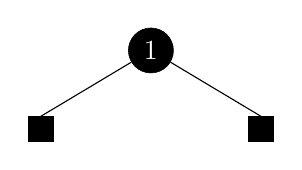
\begin{tikzpicture}[-,>=stealth',level/.style={sibling distance = 2.8cm/#1, level distance = 1cm},
                    edge from parent path={(\tikzparentnode) -- (\tikzchildnode.north)}]
                    \node 
                    [black_node] {$1$}
                    child { node [nil] {} }
                    child { node [nil] {} }
                    ; 
                \end{tikzpicture}
            \end{center}
        \end{minipage}
        \onslide<2>{
            \begin{minipage}{.1\textwidth}
                \begin{center}
                    \tikz \draw[-latex] (0,0) -- (1,0);
                \end{center}
            \end{minipage}
            \begin{minipage}{.4\textwidth}
                \begin{center}
                    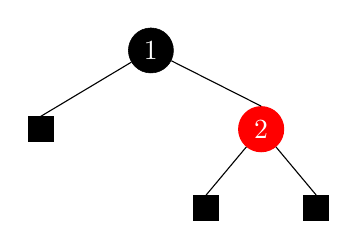
\begin{tikzpicture}[-,>=stealth',level/.style={sibling distance = 2.8cm/#1, level distance = 1cm},
                        edge from parent path={(\tikzparentnode) -- (\tikzchildnode.north)}]
                    \node 
                    [black_node] {$1$}
                    child { node [nil] {} }
                    child { 
                        node [red_node] {$2$} 
                        child { node [nil] {} }
                        child { node [nil] {} }
                    }
                    ; 
                    \end{tikzpicture}
                \end{center}
            \end{minipage}
        }
    \end{center}
\end{frame}

\begin{frame}[fragile]{Red-Black Tree: Example}
    \begin{center}
        \begin{minipage}{.4\textwidth}
            \begin{center}
                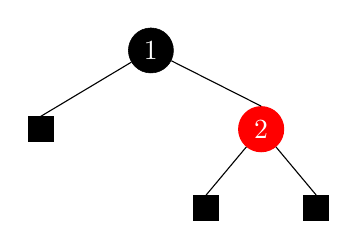
\begin{tikzpicture}[-,>=stealth',level/.style={sibling distance = 2.8cm/#1, level distance = 1cm},
                    edge from parent path={(\tikzparentnode) -- (\tikzchildnode.north)}]
                    \node 
                    [black_node] {$1$}
                    child { node [nil] {} }
                    child { 
                        node [red_node] {$2$} 
                        child { node [nil] {} }
                        child { node [nil] {} }
                    }
                    ; 
                \end{tikzpicture}
            \end{center}
        \end{minipage}
        \onslide<2>{
            \begin{minipage}{.1\textwidth}
                \begin{center}
                    \tikz \draw[-latex] (0,0) -- (1,0);
                \end{center}
            \end{minipage}
            \begin{minipage}{.4\textwidth}
                \begin{center}
                    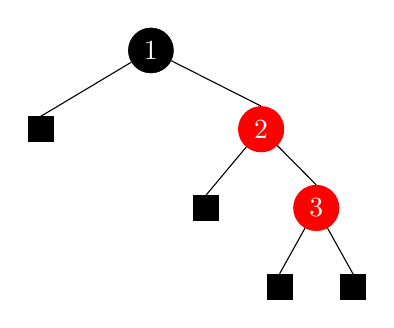
\begin{tikzpicture}[-,>=stealth',level/.style={sibling distance = 2.8cm/#1, level distance = 1cm},
                        edge from parent path={(\tikzparentnode) -- (\tikzchildnode.north)}]
                    \node 
                    [black_node] {$1$}
                    child { node [nil] {} }
                    child { 
                        node [red_node] {$2$} 
                        child { node [nil] {} }
                        child { 
                            node [red_node] {$3$} 
                            child { node [nil] {} }
                            child { node [nil] {} }
                        }
                    }
                    ; 
                    \end{tikzpicture}
                    \newline
                    \hfil
                    \newline
                    \textib{Case: Right-Right}
                \end{center}
            \end{minipage}
        }
    \end{center}
\end{frame}

\begin{frame}[fragile]{Red-Black Tree: Example}
    \begin{center}
        \begin{minipage}{.4\textwidth}
            \begin{center}
                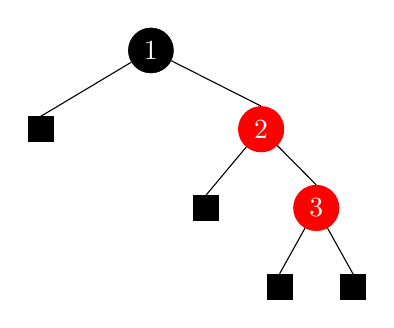
\begin{tikzpicture}[-,>=stealth',level/.style={sibling distance = 2.8cm/#1, level distance = 1cm},
                    edge from parent path={(\tikzparentnode) -- (\tikzchildnode.north)}]
                    \node 
                    [black_node] {$1$}
                    child { node [nil] {} }
                    child { 
                        node [red_node] {$2$} 
                        child { node [nil] {} }
                        child { 
                            node [red_node] {$3$} 
                            child { node [nil] {} }
                            child { node [nil] {} }
                        }
                    }
                    ; 
                \end{tikzpicture}
                \newline
                \hfil
                \newline
                \textib{Case: Right-Right}
            \end{center}
        \end{minipage}
        \onslide<2>{
            \begin{minipage}{.1\textwidth}
                \begin{center}
                    \tikz \draw[-latex] (0,0) -- (1,0);
                \end{center}
            \end{minipage}
            \begin{minipage}{.4\textwidth}
                \begin{center}
                    \begin{tikzpicture}[-,>=stealth',level/.style={sibling distance = 2.8cm/#1, level distance = 1cm},
                        edge from parent path={(\tikzparentnode) -- (\tikzchildnode.north)}]
                        \node 
                        [black_node] {$2$}
                        child { 
                            node [red_node] {$1$} 
                            child { node [nil] {} }
                            child { node [nil] {} }
                        }
                        child { 
                            node [red_node] {$3$} 
                            child { node [nil] {} }
                            child { node [nil] {} }
                        }
                        ; 
                    \end{tikzpicture}
                \end{center}
            \end{minipage}
            }
    \end{center}
\end{frame}

\begin{frame}[fragile]{Red-Black Tree: Example}
    \begin{center}
        \begin{minipage}{.4\textwidth}
            \begin{center}
                \begin{tikzpicture}[-,>=stealth',level/.style={sibling distance = 2.8cm/#1, level distance = 1cm},
                    edge from parent path={(\tikzparentnode) -- (\tikzchildnode.north)}]
                    \node 
                    [black_node] {$2$}
                    child { 
                        node [red_node] {$1$} 
                        child { node [nil] {} }
                        child { node [nil] {} }
                    }
                    child { 
                        node [red_node] {$3$} 
                        child { node [nil] {} }
                        child { node [nil] {} }
                    }
                    ; 
                \end{tikzpicture}
            \end{center}
        \end{minipage}
        \onslide<2>{
            \begin{minipage}{.1\textwidth}
                \begin{center}
                    \tikz \draw[-latex] (0,0) -- (1,0);
                \end{center}
            \end{minipage}
            \begin{minipage}{.4\textwidth}
                \begin{center}
                    \begin{tikzpicture}[-,>=stealth',level/.style={sibling distance = 2.8cm/#1, level distance = 1cm},
                        edge from parent path={(\tikzparentnode) -- (\tikzchildnode.north)}]
                        \node 
                        [black_node] {$2$}
                        child { 
                            node [red_node] {$1$} 
                            child { node [nil] {} }
                            child { node [nil] {} }
                        }
                        child { 
                            node [red_node] {$3$} 
                            child { node [nil] {} }
                            child { 
                                node [red_node] {$4$} 
                                child { node [nil] {} }
                                child { node [nil] {} }
                            }
                        }
                        ; 
                    \end{tikzpicture}
                    \newline
                    \hfil
                    \newline
                    \textib{Case: Recolor}
                \end{center}
            \end{minipage}
            }
    \end{center}
\end{frame}

\begin{frame}[fragile]{Red-Black Tree: Example}
    \begin{center}
        \begin{minipage}{.4\textwidth}
            \begin{center}
                \begin{tikzpicture}[-,>=stealth',level/.style={sibling distance = 2.8cm/#1, level distance = 1cm},
                    edge from parent path={(\tikzparentnode) -- (\tikzchildnode.north)}]
                    \node 
                    [black_node] {$2$}
                    child { 
                        node [red_node] {$1$} 
                        child { node [nil] {} }
                        child { node [nil] {} }
                    }
                    child { 
                        node [red_node] {$3$} 
                        child { node [nil] {} }
                        child { 
                            node [red_node] {$4$} 
                            child { node [nil] {} }
                            child { node [nil] {} }
                        }
                    }
                    ; 
                \end{tikzpicture}
                \newline
                \hfil
                \newline
                \textib{Case: Recolor}
            \end{center}
        \end{minipage}
        \onslide<2>{
            \begin{minipage}{.1\textwidth}
                \begin{center}
                    \tikz \draw[-latex] (0,0) -- (1,0);
                \end{center}
            \end{minipage}
            \begin{minipage}{.4\textwidth}
                \begin{center}
                    \begin{tikzpicture}[-,>=stealth',level/.style={sibling distance = 2.8cm/#1, level distance = 1cm},
                        edge from parent path={(\tikzparentnode) -- (\tikzchildnode.north)}]
                        \node 
                        [black_node] {$2$}
                        child { 
                            node [black_node] {$1$} 
                            child { node [nil] {} }
                            child { node [nil] {} }
                        }
                        child { 
                            node [black_node] {$3$} 
                            child { node [nil] {} }
                            child { 
                                node [red_node] {$4$} 
                                child { node [nil] {} }
                                child { node [nil] {} }
                            }
                        }
                        ; 
                    \end{tikzpicture}
                \end{center}
            \end{minipage}
            }
    \end{center}
\end{frame}

\begin{frame}[fragile]{Red-Black Tree: Example}
    \begin{center}
        \begin{minipage}{.4\textwidth}
            \begin{center}
                \begin{tikzpicture}[-,>=stealth',level/.style={sibling distance = 2.8cm/#1, level distance = 1cm},
                    edge from parent path={(\tikzparentnode) -- (\tikzchildnode.north)}]
                    \node 
                    [black_node] {$2$}
                    child { 
                        node [black_node] {$1$} 
                        child { node [nil] {} }
                        child { node [nil] {} }
                    }
                    child { 
                        node [black_node] {$3$} 
                        child { node [nil] {} }
                        child { 
                            node [red_node] {$4$} 
                            child { node [nil] {} }
                            child { node [nil] {} }
                        }
                    }
                    ; 
                \end{tikzpicture}
            \end{center}
        \end{minipage}
        \onslide<2>{
            \begin{minipage}{.1\textwidth}
                \begin{center}
                    \tikz \draw[-latex] (0,0) -- (1,0);
                \end{center}
            \end{minipage}
            \begin{minipage}{.4\textwidth}
                \begin{center}
                    \begin{tikzpicture}[-,>=stealth',level/.style={sibling distance = 2.8cm/#1, level distance = 1cm},
                        edge from parent path={(\tikzparentnode) -- (\tikzchildnode.north)}]
                        \node 
                        [black_node] {$2$}
                        child { 
                            node [black_node] {$1$} 
                            child { node [nil] {} }
                            child { node [nil] {} }
                        }
                        child { 
                            node [black_node] {$3$} 
                            child { node [nil] {} }
                            child { 
                                node [red_node] {$4$} 
                                child { node [nil] {} }
                                child { 
                                    node [red_node] {$5$} 
                                    child { node [nil] {} }
                                    child { node [nil] {} }
                                }
                            }
                        }
                        ; 
                    \end{tikzpicture}
                    \newline
                    \hfil
                    \newline
                    \textib{Case: Right-Right}
                \end{center}
            \end{minipage}
            }
    \end{center}
\end{frame}

\begin{frame}[fragile]{Red-Black Tree: Example}
    \begin{center}
        \begin{minipage}{.4\textwidth}
            \begin{center}
                \begin{tikzpicture}[-,>=stealth',level/.style={sibling distance = 2.8cm/#1, level distance = 1cm},
                    edge from parent path={(\tikzparentnode) -- (\tikzchildnode.north)}]
                    \node 
                    [black_node] {$2$}
                    child { 
                        node [black_node] {$1$} 
                        child { node [nil] {} }
                        child { node [nil] {} }
                    }
                    child { 
                        node [black_node] {$3$} 
                        child { node [nil] {} }
                        child { 
                            node [red_node] {$4$} 
                            child { node [nil] {} }
                            child { 
                                node [red_node] {$5$} 
                                child { node [nil] {} }
                                child { node [nil] {} }
                            }
                        }
                    }
                    ; 
                \end{tikzpicture}
                \newline
                \hfil
                \newline
                \textib{Case: Right-Right}
            \end{center}
        \end{minipage}
        \onslide<2>{
            \begin{minipage}{.1\textwidth}
                \begin{center}
                    \tikz \draw[-latex] (0,0) -- (1,0);
                \end{center}
            \end{minipage}
            \begin{minipage}{.4\textwidth}
                \begin{center}
                    \begin{tikzpicture}[-,>=stealth',level/.style={sibling distance = 2.8cm/#1, level distance = 1cm},
                        edge from parent path={(\tikzparentnode) -- (\tikzchildnode.north)}]
                        \node 
                        [black_node] {$2$}
                        child { 
                            node [black_node] {$1$} 
                            child { node [nil] {} }
                            child { node [nil] {} }
                        }
                        child { 
                            node [black_node] {$4$} 
                            child { 
                                node [red_node] {$3$} 
                                child { node [nil] {} }
                                child { node [nil] {} }
                            }
                            child { 
                                node [red_node] {$5$} 
                                child { node [nil] {} }
                                child { node [nil] {} }
                            }
                        }
                        ; 
                    \end{tikzpicture}
                \end{center}
            \end{minipage}
            }
    \end{center}
\end{frame}

\begin{frame}[fragile]{Red-Black Tree: Example}
    \begin{center}
        \begin{minipage}{.4\textwidth}
            \begin{center}
                \begin{tikzpicture}[-,>=stealth',level/.style={sibling distance = 2.8cm/#1, level distance = 1cm},
                    edge from parent path={(\tikzparentnode) -- (\tikzchildnode.north)}]
                    \node 
                    [black_node] {$2$}
                    child { 
                        node [black_node] {$1$} 
                        child { node [nil] {} }
                        child { node [nil] {} }
                    }
                    child { 
                        node [black_node] {$4$} 
                        child { 
                            node [red_node] {$3$} 
                            child { node [nil] {} }
                            child { node [nil] {} }
                        }
                        child { 
                            node [red_node] {$5$} 
                            child { node [nil] {} }
                            child { node [nil] {} }
                        }
                    }
                    ; 
                \end{tikzpicture}
            \end{center}
        \end{minipage}
        \onslide<2>{
            \begin{minipage}{.1\textwidth}
                \begin{center}
                    \tikz \draw[-latex] (0,0) -- (1,0);
                \end{center}
            \end{minipage}
            \begin{minipage}{.4\textwidth}
                \begin{center}
                    \begin{tikzpicture}[-,>=stealth',level/.style={sibling distance = 2.8cm/#1, level distance = 1cm},
                        edge from parent path={(\tikzparentnode) -- (\tikzchildnode.north)}]
                        \node 
                        [black_node] {$2$}
                        child { 
                            node [black_node] {$1$} 
                            child { node [nil] {} }
                            child { node [nil] {} }
                        }
                        child { 
                            node [black_node] {$4$} 
                            child { 
                                node [red_node] {$3$} 
                                child { node [nil] {} }
                                child { node [nil] {} }
                            }
                            child { 
                                node [red_node] {$5$} 
                                child { node [nil] {} }
                                child { 
                                    node [red_node] {$6$} 
                                    child { node [nil] {} }
                                    child { node [nil] {} }
                                }
                            }
                        }
                        ; 
                    \end{tikzpicture}
                    \newline
                    \hfil
                    \newline
                    \textib{Case: Recolor}
                \end{center}
            \end{minipage}
            }
    \end{center}
\end{frame}

\begin{frame}[fragile]{Red-Black Tree: Example}
    \begin{center}
        \begin{minipage}{.4\textwidth}
            \begin{center}
                \begin{tikzpicture}[-,>=stealth',level/.style={sibling distance = 2.8cm/#1, level distance = 1cm},
                    edge from parent path={(\tikzparentnode) -- (\tikzchildnode.north)}]
                    \node 
                    [black_node] {$2$}
                    child { 
                        node [black_node] {$1$} 
                        child { node [nil] {} }
                        child { node [nil] {} }
                    }
                    child { 
                        node [black_node] {$4$} 
                        child { 
                            node [red_node] {$3$} 
                            child { node [nil] {} }
                            child { node [nil] {} }
                        }
                        child { 
                            node [red_node] {$5$} 
                            child { node [nil] {} }
                            child { 
                                node [red_node] {$6$} 
                                child { node [nil] {} }
                                child { node [nil] {} }
                            }
                        }
                    }
                    ; 
                \end{tikzpicture}
                \newline
                \hfil
                \newline
                \textib{Case: Recolor}
            \end{center}
        \end{minipage}
        \onslide<2>{
            \begin{minipage}{.1\textwidth}
                \begin{center}
                    \tikz \draw[-latex] (0,0) -- (1,0);
                \end{center}
            \end{minipage}
            \begin{minipage}{.4\textwidth}
                \begin{center}
                    \begin{tikzpicture}[-,>=stealth',level/.style={sibling distance = 2.8cm/#1, level distance = 1cm},
                        edge from parent path={(\tikzparentnode) -- (\tikzchildnode.north)}]
                        \node 
                        [black_node] {$2$}
                        child { 
                            node [black_node] {$1$} 
                            child { node [nil] {} }
                            child { node [nil] {} }
                        }
                        child { 
                            node [red_node] {$4$} 
                            child { 
                                node [black_node] {$3$} 
                                child { node [nil] {} }
                                child { node [nil] {} }
                            }
                            child { 
                                node [black_node] {$5$} 
                                child { node [nil] {} }
                                child { 
                                    node [red_node] {$6$} 
                                    child { node [nil] {} }
                                    child { node [nil] {} }
                                }
                            }
                        }
                        ; 
                    \end{tikzpicture}
                \end{center}
            \end{minipage}
            }
    \end{center}
\end{frame}

\begin{frame}[fragile]{Red-Black Tree: Example}
    \begin{center}
        \begin{minipage}{.4\textwidth}
            \begin{center}
                \begin{tikzpicture}[-,>=stealth',level/.style={sibling distance = 2.8cm/#1, level distance = 1cm},
                    edge from parent path={(\tikzparentnode) -- (\tikzchildnode.north)}]
                    \node 
                    [black_node] {$2$}
                    child { 
                        node [black_node] {$1$} 
                        child { node [nil] {} }
                        child { node [nil] {} }
                    }
                    child { 
                        node [red_node] {$4$} 
                        child { 
                            node [black_node] {$3$} 
                            child { node [nil] {} }
                            child { node [nil] {} }
                        }
                        child { 
                            node [black_node] {$5$} 
                            child { node [nil] {} }
                            child { 
                                node [red_node] {$6$} 
                                child { node [nil] {} }
                                child { node [nil] {} }
                            }
                        }
                    }
                    ; 
                \end{tikzpicture}
            \end{center}
        \end{minipage}
        \onslide<2>{
            \begin{minipage}{.1\textwidth}
                \begin{center}
                    \tikz \draw[-latex] (0,0) -- (1,0);
                \end{center}
            \end{minipage}
            \begin{minipage}{.4\textwidth}
                \begin{center}
                    \begin{tikzpicture}[-,>=stealth',level/.style={sibling distance = 2.8cm/#1, level distance = 1cm},
                        edge from parent path={(\tikzparentnode) -- (\tikzchildnode.north)}, scale=0.8]
                        \node 
                        [black_node, scale=0.8] {$2$}
                        child { 
                            node [black_node, scale=0.8] {$1$} 
                            child { node [nil, scale=0.8] {} }
                            child { node [nil, scale=0.8] {} }
                        }
                        child { 
                            node [red_node, scale=0.8] {$4$} 
                            child { 
                                node [black_node, scale=0.8] {$3$} 
                                child { node [nil, scale=0.8] {} }
                                child { node [nil, scale=0.8] {} }
                            }
                            child { 
                                node [black_node, scale=0.8] {$5$} 
                                child { node [nil, scale=0.8] {} }
                                child { 
                                    node [red_node, scale=0.8] {$6$} 
                                    child { node [nil, scale=0.8] {} }
                                    child { 
                                        node [red_node, scale=0.8] {$7$} 
                                        child { node [nil, scale=0.8] {} }
                                        child { node [nil, scale=0.8] {} }
                                    }
                                }
                            }
                        }
                        ; 
                    \end{tikzpicture}
                    \newline
                    \hfil
                    \newline
                    \textib{Case: Right-Right}
                \end{center}
            \end{minipage}
            }
    \end{center}
\end{frame}

\begin{frame}[fragile]{Red-Black Tree: Example}
    \begin{center}
        \begin{minipage}{.35\textwidth}
            \begin{center}
                \begin{tikzpicture}[-,>=stealth',level/.style={sibling distance = 2.8cm/#1, level distance = 1cm},
                    edge from parent path={(\tikzparentnode) -- (\tikzchildnode.north)}, scale=0.8]
                    \node 
                    [black_node, scale=0.8] {$2$}
                    child { 
                        node [black_node, scale=0.8] {$1$} 
                        child { node [nil, scale=0.8] {} }
                        child { node [nil, scale=0.8] {} }
                    }
                    child { 
                        node [red_node, scale=0.8] {$4$} 
                        child { 
                            node [black_node, scale=0.8] {$3$} 
                            child { node [nil, scale=0.8] {} }
                            child { node [nil, scale=0.8] {} }
                        }
                        child { 
                            node [black_node, scale=0.8] {$5$} 
                            child { node [nil, scale=0.8] {} }
                            child { 
                                node [red_node, scale=0.8] {$6$} 
                                child { node [nil, scale=0.8] {} }
                                child { 
                                    node [red_node, scale=0.8] {$7$} 
                                    child { node [nil, scale=0.8] {} }
                                    child { node [nil, scale=0.8] {} }
                                }
                            }
                        }
                    }
                    ; 
                \end{tikzpicture}
            \end{center}
        \end{minipage}
        \onslide<2>{
            \begin{minipage}{.08\textwidth}
                \begin{center}
                    \tikz \draw[-latex] (0,0) -- (1,0);
                \end{center}
            \end{minipage}
            \begin{minipage}{.45\textwidth}
                \begin{center}
                    \begin{tikzpicture}[-,>=stealth',level/.style={sibling distance = 4cm/#1, level distance = 1cm},
                        edge from parent path={(\tikzparentnode) -- (\tikzchildnode.north)}, scale=0.8]
                        \node 
                        [black_node, scale=0.8] {$2$}
                        child { 
                            node [black_node, scale=0.8] {$1$} 
                            child { node [nil, scale=0.8] {} }
                            child { node [nil, scale=0.8] {} }
                        }
                        child { 
                            node [red_node, scale=0.8] {$4$} 
                            child { 
                                node [black_node, scale=0.8] {$3$} 
                                child { node [nil, scale=0.8] {} }
                                child { node [nil, scale=0.8] {} }
                            }
                            child { 
                                node [black_node, scale=0.8] {$6$} 
                                child { 
                                    node [red_node, scale=0.8] {$5$} 
                                    child { node [nil, scale=0.6] {} }
                                    child { node [nil, scale=0.6] {} }
                                }
                                child { 
                                    node [red_node, scale=0.8] {$7$} 
                                    child { node [nil, scale=0.6] {} }
                                    child { node [nil, scale=0.6] {} }
                                }
                            }
                        }
                        ; 
                    \end{tikzpicture}
                \end{center}
            \end{minipage}
            }
    \end{center}
\end{frame}

\begin{frame}{Applications}
    Red-Black Trees have a variety of applications. Some include:
    \begin{enumerate}[label=\textit{(\roman*)}]
        \item Database indexing 
        \item<2-> Linux CPU scheduler
        \item<3-> Linux page tables
        \item<4-> C++'s \texttt{std::map}
        \item<5-> Graph algorithms (Dijkstra, MST)
    \end{enumerate}
\end{frame}

\begin{frame}{End}
    \begin{center}
        Thank you!
    \end{center}
\end{frame}


\begin{frame}{Appendix}
\end{frame}


% ===== COROLLARIES =====
\begin{frame}{Corollaries}
    \proposition{
        If a node $n$ has exactly one child, $c$, then 
        \textnormal{\textbf{(a)}} $c$ is \red,
        \textnormal{\textbf{(b)}} $n$ is \textib{black}, and
        \textnormal{\textbf{(c)}} $c$ has no children.
    }
    \textit{Proof.}
    Suppose we have a valid red-black tree. Consider a node $n$ with exactly one child. 
    Without loss of generality, choose $n$'s left node to be the child and call it $c$.
    \begin{enumerate}[label=\textbf{(\alph*)}]
        \item<2-> $n$ passes through no \textib{black} nodes on the right side by assumption. If $c$ were 
            \textib{black}, then $n$ would pass through $1$ \textib{black} node, a contradiction 
            since this violates \textit{(iv)}.
        \item<3-> By \textbf{(a)}, $n$'s child is \red and by \textit{(iii)}, $n$ is \textib{black}.
        \item <4-> Since $n$ passes through no \textib{black} nodes on the right side by assumption,
            $n$ cannot pass through any \textib{black} nodes on the left side by \textit{(iv)}. Then,
            since $c$ is \red by \textbf{(a)}, $c$ has only nil nodes, which are \textib{black} by
            \textit{(ii)}.
        \end{enumerate}
    \onslide<4->{\qed}


    % \textbf{(a)} Suppose we have a valid red-black tree. Consider a node $n$ with exactly one child. 
    % Without loss of generality, choose $n$'s left node to be the child and call it $c$. 
    % Then, $n$ passes through no \textib{black} nodes on the right side. If $c$ were \textib{black}, then $n$ would 
    % pass through $1$ \textib{black} node, a contradiction since this violates \textit{(iv)}.
    % \newline
    % \onslide<2->{
    %     \textbf{(b)} By \textbf{(a)}, $n$'s child is \red and by \textit{(iii)}, $n$ is \textib{black}.
    % }
    % \newline
    % \onslide<3->{
    %     \textbf{(c)} By \textit{(iii)}, $c$ must have \textib{black} children. But since $n$ passes
    %     through no \textib{black} nodes on the right side, by \textit{(iv)}, $n$ cannot pass through
    %     any \textib{black} nodes on the left side. Since $c$ is \red by \textbf{(a)}, $c$ must have
    %     no children.
    %     \qed
    % }
\end{frame}

\begin{frame}{Height of a Red-Black Tree}
    \thm{
    A red-black tree with $n$ nodes has a height $h$ that is ${\cal{O}} (\log n)$.
    }
    \textit{Proof.}
    Suppose we have an arbitrary red-black tree with $n$ nodes.
    \newline
    \onslide<2->{$|$Shortest path (root $\to$ leaf)$|$ $b$ contains exclusively \textib{black} nodes $\implies b \leq h$.}
    \newline
    \onslide<3->{$|$Longest path (root $\to$ leaf)$|$ alternates between \red and \textib{black} nodes $\implies h \leq 2b$.}
    \newline
    \onslide<4->{Then $b \leq h \leq 2b$. $(*)$}
    \newline
    \onslide<5->{There are $2^b - 1 \leq n$ nodes in the tree $\implies b \leq \log(n + 1)$.}
    \newline
    \onslide<6->{Then, from $(*)$ we get
        \newline
        \[
            b \leq \log(n + 1) \leq h \leq 2b \leq 2\log(n + 1)
            \iff \log(n + 1) \leq h \leq 2\log(n + 1)
        \]
    }
    \newline
    \onslide<7->{
        $\implies h$ is ${\cal{O}} (\log n)$.
        \qed
    }
\end{frame}

\begin{frame}{Height of a Red-Black Tree (Written Proof)}
    \thm{
        A red-black tree with $n$ nodes has a height $h$ that is ${\cal{O}}(\log n)$.
    }
    \textit{Proof.}
    Suppose we have an arbitrary red-black tree with $n$ nodes. Then, the length of the shortest 
    path $b$ from root to leaf contains exclusively \textib{black} nodes (by 
    \textit{(iv)}), so the height $h$ must be at least $b$. Conversely, the length of the longest 
    path from root to leaf contains an alternating sequence of \red and \textib{black} nodes 
    (by \textit{(iii)}), with length at most $2b$. Note that there are at least $2^b - 1$ nodes in the 
    tree. Solving for $b$, we get $b \leq \log(n + 1)$. Since $b \leq h$, we have that the height 
    of the red-black tree must be at least $\log(n + 1)$. Then, we get 
    \[b \leq \log(n + 1) \leq h \leq 2b \leq 2\log(n + 1)\]
    or
    \[\log(n + 1) \leq h \leq 2\log(n + 1)\]
    thus the height of a red-black tree with $n$ nodes is ${\cal{O}} (\log n)$.
    \qed
\end{frame}

\end{document}
